\documentclass[12pt,a4paper]{report}

% PACKAGES
\usepackage[T1]{fontenc}
\usepackage[utf8]{inputenc}
\usepackage[english]{babel}
\usepackage{lmodern}
\usepackage{geometry}
\usepackage{graphicx}
\usepackage{xcolor}
\usepackage{titlesec}
\usepackage{fancyhdr}
\usepackage{setspace}
\usepackage{booktabs}
\usepackage{array}
\usepackage{enumitem}
\usepackage{hyperref}
\usepackage{microtype}
\usepackage{parskip}
\usepackage{mdframed}
\usepackage{tikz}
\usetikzlibrary{positioning, shapes.geometric, arrows.meta, calc, fit}
\usepackage{amsmath}
\usepackage{tcolorbox}
\usepackage{float}
\usepackage{makecell}
\usepackage{listings}
\usepackage{longtable}

% PAGE GEOMETRY
\geometry{a4paper,left=2.5cm,right=2.5cm,top=2.5cm,bottom=2.5cm,headheight=15pt}

% COLOURS
\definecolor{darkblue}{HTML}{002366} % Professional Navy Blue
\definecolor{darkbg}{HTML}{0f172a}
\definecolor{emerald}{HTML}{10b981}
\definecolor{teal}{HTML}{0d9488}
\definecolor{gold}{HTML}{d4af37}
\definecolor{goldlt}{HTML}{b8920a}
\definecolor{slategray}{HTML}{64748b}
\definecolor{lightblue}{HTML}{2563eb}
\definecolor{warshgreen}{HTML}{059669}
\definecolor{warnred}{HTML}{ea580c}
\definecolor{violet}{HTML}{7c3aed}
\definecolor{cardbg}{HTML}{f0f9ff}
\definecolor{tealbg}{HTML}{f0fdfa}
\definecolor{goldbg}{HTML}{fffbeb}
\definecolor{redbg}{HTML}{fff7ed}

% HYPERREF
\hypersetup{
    colorlinks=true,linkcolor=black,urlcolor=black,citecolor=black,
    pdftitle={Tahkik Server --- Technical Report},
    pdfauthor={Benhadjer Mohamed, Bouziani Alaa Eddine}
}

% SECTION TITLE STYLES
\titleformat{\chapter}[block]
  {\normalfont\LARGE\bfseries\color{darkblue}}
  {\thechapter.}{12pt}{}
  [\vspace{2pt}\color{darkblue}\rule{\textwidth}{1.5pt}]

\titleformat{\section}
  {\normalfont\large\bfseries\color{darkblue}}
  {\thesection}{10pt}{}

\titleformat{\subsection}
  {\normalfont\normalsize\bfseries\color{darkblue}}
  {\thesubsection}{8pt}{}

\titlespacing*{\chapter}{0pt}{0pt}{20pt}

% HEADER / FOOTER
\pagestyle{fancy}
\fancyhf{}
\fancyhead[L]{\small\color{black}\textit{Tahkik --- AI-Powered Quran Recitation}}
\fancyhead[R]{\small\color{black}L3 Computer Science --- 2025/2026}
\fancyfoot[C]{\small\color{black}\thepage}
\renewcommand{\headrulewidth}{0.4pt}
\renewcommand{\headrule}{\hbox to\headwidth{\color{black}\leaders\hrule height \headrulewidth\hfill}}

% TCOLORBOX STYLES
\tcbuselibrary{skins,breakable}

\newtcolorbox{emeraldbox}[1][]{
  enhanced, colback=white, colframe=black,
  fonttitle=\bfseries\color{white}, colbacktitle=black,
  attach boxed title to top left={yshift=-2mm,xshift=6mm},
  boxed title style={sharp corners}, sharp corners, breakable, #1
}

\newtcolorbox{goldbox}[1][]{
  enhanced, colback=white, colframe=black,
  fonttitle=\bfseries\color{white}, colbacktitle=black,
  attach boxed title to top left={yshift=-2mm,xshift=6mm},
  boxed title style={sharp corners}, sharp corners, breakable, #1
}

\newtcolorbox{warnbox}[1][]{
  enhanced, colback=white, colframe=black,
  fonttitle=\bfseries\color{white}, colbacktitle=black,
  attach boxed title to top left={yshift=-2mm,xshift=6mm},
  boxed title style={sharp corners}, sharp corners, breakable, #1
}

\newtcolorbox{infobox}[1][]{
  enhanced, colback=white, colframe=black,
  fonttitle=\bfseries\color{white}, colbacktitle=black,
  attach boxed title to top left={yshift=-2mm,xshift=6mm},
  boxed title style={sharp corners}, sharp corners, breakable, #1
}

% CUSTOM PHASE BLOCK (Compatible with part 2)
\newcommand{\phaseblock}[3][]{%
  \begin{tcolorbox}[
    enhanced, colback=white, colframe=black,
    leftrule=5pt, sharp corners, before upper={\parindent0pt}, #1
  ]
  {\bfseries\color{black}#2}\\[4pt]
  \small #3
  \end{tcolorbox}%
}

% SCREENSHOT PLACEHOLDER
\newcommand{\screenshotplaceholder}[2]{%
  \begin{figure}[H]
    \centering
    \fbox{\parbox{#1\textwidth}{\centering\vspace{3cm}
      \textit{Screenshot: #2}\vspace{3cm}}}
  \end{figure}%
}

% LOGO PLACEHOLDER
\newcommand{\logoplaceholder}[1]{%
  \fbox{\parbox{1.5cm}{\centering\vspace{0.5cm}
    \scriptsize\textit{Logo: #1}\vspace{0.5cm}}}%
}

% CODE LISTING STYLE
\lstset{
  basicstyle=\ttfamily\small,
  backgroundcolor=\color{white},
  frame=single,
  rulecolor=\color{black},
  breaklines=true,
  numbers=left,
  numberstyle=\tiny\color{black},
  tabsize=2
}

\onehalfspacing

\begin{document}

% COVER PAGE
\begin{titlepage}
\newgeometry{left=2cm,right=2cm,top=2cm,bottom=2cm}

\begin{tikzpicture}[remember picture, overlay]
  \fill[gold] ([yshift=-0.5cm]current page.north west) rectangle ([yshift=-0.58cm]current page.north east);
  \fill[teal!70!black] (current page.south west) rectangle ([yshift=0.08cm]current page.south east);
\end{tikzpicture}

\vspace*{1.5cm}

\begin{center}
  {\color{darkbg}\large\bfseries University of Yahia Fares Medea}\\[5pt]
  {\color{goldlt}\normalsize Faculty of Sciences \& Technology}\\[3pt]
  {\color{slategray}\small Department of Computer Science}\\[2pt]
  {\color{slategray}\small Academic Year 2025 / 2026}
\end{center}

\vspace{1.5cm}

\begin{center}
  
\begin{tikzpicture}
    \node[
      draw=emerald!80!black, fill=emerald!15!white,
      rounded corners=10pt, inner sep=7pt,
      font=\small\bfseries, text=emerald!70!black
    ] {Go \(\cdot\) Python \(\cdot\) FastAPI \(\cdot\) Whisper \(\cdot\) HF Spaces};
  \end{tikzpicture}
\end{center}

\vspace{1.5cm}

\begin{center}
  {\LARGE\bfseries\color{darkbg} Tahkik Inference Server}\\[15pt]
  {\huge\bfseries\color{teal} Technical Report}\\[10pt]
  {\Large\bfseries\color{teal} Server Architecture, API \& Deployment}
\end{center}

\vspace{2cm}

\begin{center}
  {\color{gold}\rule{0.55\textwidth}{1.2pt}}
\end{center}

\vspace{2cm}

\begin{center}
  \renewcommand{\arraystretch}{1.5}
  \begin{tabular}{cc}
    {\large\bfseries Benhadjer Mohamed} & {\large\bfseries Bouziani Alaa Eddine} \\
    {\small\color{slategray} Group 2} & {\small\color{slategray} Group 2} \\
    {\small\color{slategray} L3 Computer Science} & {\small\color{slategray} L3 Computer Science}
  \end{tabular}
\end{center}

\vfill
\restoregeometry
\end{titlepage}

% REDEFINE COLORS FOR CONTENT (All in Black, titles already Dark Blue)
\definecolor{teal}{HTML}{000000}
\definecolor{gold}{HTML}{000000}
\definecolor{emerald}{HTML}{000000}
\definecolor{slategray}{HTML}{000000}
\definecolor{tealbg}{HTML}{FFFFFF}
\definecolor{goldbg}{HTML}{FFFFFF}
\definecolor{cardbg}{HTML}{FFFFFF}
\definecolor{redbg}{HTML}{FFFFFF}
\definecolor{warnred}{HTML}{000000}


% TABLE OF CONTENTS
\tableofcontents
\newpage

%% --- PART 1 ENDS HERE --- input part 2
% ═══════════════════════════════════════════════════════════════════════════════
% CHAPTER 1: INTRODUCTION
% ═══════════════════════════════════════════════════════════════════════════════
\chapter{Introduction}

This technical report documents the server-side infrastructure of the Tahkik project --- an AI-powered Quranic recitation analysis system specializing in the Warsh 'an Nafi' riwaya. The server bridges the Flutter mobile application with the Whisper-based inference model, handling audio uploads, forwarding them to the machine learning backend, and returning structured transcription results.

The system is composed of two primary components: a Go HTTP API gateway that receives client requests and a Python inference backend (deployed as a Hugging Face Space) that runs the fine-tuned Whisper model. This report covers the architecture, component details, data pipeline, API contracts, deployment procedures, and troubleshooting.

% ═══════════════════════════════════════════════════════════════════════════════
% CHAPTER 2: SYSTEM ARCHITECTURE
% ═══════════════════════════════════════════════════════════════════════════════
\chapter{System Architecture}

\section{System Overview}

The Tahkik server follows a proxy architecture where the Go API server acts as a gateway between the mobile client and the ML inference backend. This design keeps authentication tokens server-side and allows swapping inference backends without modifying the Flutter codebase.

\begin{figure}[H]
\centering
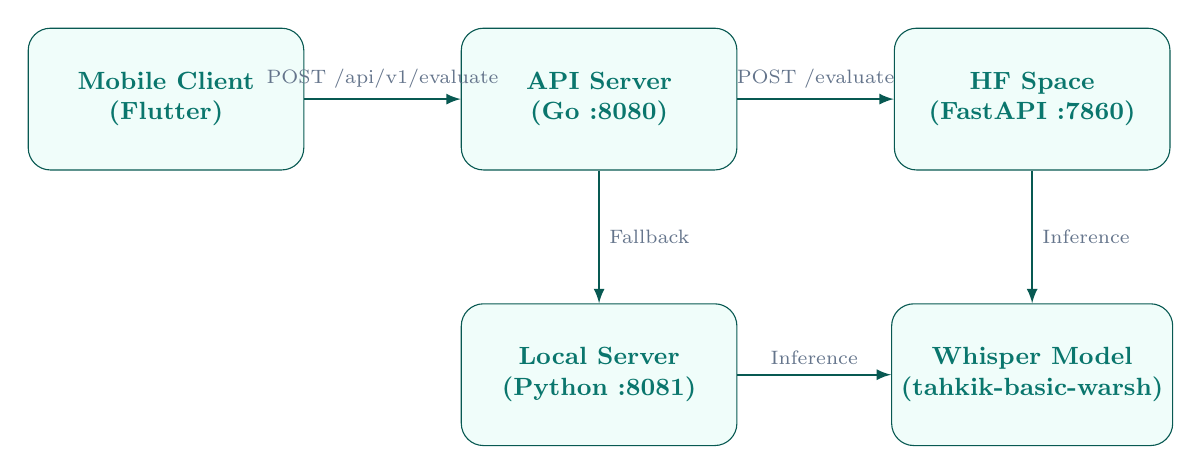
\begin{tikzpicture}[
  component/.style={
    draw=teal!60!black, rounded corners=8pt, minimum width=3.5cm,
    minimum height=1.8cm, fill=tealbg, font=\small\bfseries,
    text=teal!80!black, align=center
  },
  arrow/.style={-latex, thick, teal!60!black},
  label/.style={font=\scriptsize, color=slategray}
]

\node[component] (client) at (0, 0) {Mobile Client\\(Flutter)};
\node[component] (api) at (5.5, 0) {API Server\\(Go :8080)};
\node[component] (hf) at (11, 0) {HF Space\\(FastAPI :7860)};
\node[component] (model) at (11, -3.5) {Whisper Model\\(tahkik-basic-warsh)};
\node[component] (local) at (5.5, -3.5) {Local Server\\(Python :8081)};

\draw[arrow] (client) -- node[label, above] {POST /api/v1/evaluate} (api);
\draw[arrow] (api) -- node[label, above] {POST /evaluate} (hf);
\draw[arrow] (hf) -- node[label, right] {Inference} (model);
\draw[arrow] (api) -- node[label, right] {Fallback} (local);
\draw[arrow] (local) -- node[label, above] {Inference} (model);

\end{tikzpicture}
\caption{High-level system architecture}
\label{fig:architecture_overview}
\end{figure}

\section{Design Justification}

The architectural decisions were driven by the following constraints:

\begin{itemize}
    \item \textbf{Proxy Pattern:} The Go server acts as a reverse proxy, shielding the inference backend from direct client access. This enables server-side token management and backend flexibility.
    \item \textbf{Go for the API Gateway:} Go's standard library \texttt{net/http} provides a production-ready HTTP server with minimal dependencies, fast compilation, and low memory footprint.
    \item \textbf{faster-whisper (CTranslate2):} The production deployment uses \texttt{faster-whisper} with INT8 quantization, achieving approximately 4$\times$ faster inference compared to the PyTorch-based backend used during development.
    \item \textbf{Hugging Face Spaces:} Chosen for zero-infrastructure deployment with Docker SDK support, automatic scaling, and optional GPU hardware (T4/L4/A100).
    \item \textbf{WebSocket Streaming:} The \texttt{/ws/stream} endpoint enables real-time partial transcription, providing immediate user feedback during recitation without waiting for the full recording to complete.
\end{itemize}

% ═══════════════════════════════════════════════════════════════════════════════
% CHAPTER 3: COMPONENT DETAILS
% ═══════════════════════════════════════════════════════════════════════════════
\chapter{Component Details}

% --- Go API Server ---
\section{Go API Server}
\label{sec:go_api_server}

\subsection{Overview}
The Go API server is the entry point for all client requests. It listens on port 8080 (configurable via \texttt{PORT} environment variable) and exposes two endpoints: \texttt{POST /api/v1/evaluate} for audio evaluation and \texttt{GET /health} for liveness checks.

\subsection{Technology}
\begin{infobox}[title=Technology Stack]
\begin{itemize}
  \item \textbf{Language}: Go 1.26.2
  \item \textbf{Framework}: Standard library (\texttt{net/http})
  \item \textbf{Key Packages}: \texttt{encoding/json}, \texttt{mime/multipart}, \texttt{io}
\end{itemize}
\end{infobox}

\subsection{Key Implementation Details}

The server uses Go's built-in \texttt{http.NewServeMux} for routing. The evaluate handler validates the uploaded audio file (max 50\,MB, supported formats: \texttt{.wav}, \texttt{.mp3}, \texttt{.m4a}, \texttt{.flac}, \texttt{.ogg}), reads the binary data, and delegates to the ML inference client.

\begin{lstlisting}[language=Go, caption={API entry point (cmd/api/main.go)}]
func main() {
    port := os.Getenv("PORT")
    if port == "" { port = "8080" }

    mux := http.NewServeMux()
    mux.HandleFunc("/api/v1/evaluate", handlers.Evaluate)
    mux.HandleFunc("/health", func(w http.ResponseWriter, r *http.Request) {
        w.Header().Set("Content-Type", "application/json")
        w.Write([]byte(`{"status":"ok"}`))
    })

    log.Printf("Tahkik server listening on :%s", port)
    http.ListenAndServe(":"+port, mux)
}
\end{lstlisting}

\subsection{Inference Client}

The \texttt{internal/ml/inference.go} module forwards audio to the Python backend as \texttt{multipart/form-data}. It supports both local and remote backends via the \texttt{INFERENCE\_SERVER\_URL} environment variable.

\begin{lstlisting}[language=Go, caption={Inference result structure}]
type Result struct {
    Transcription    string  `json:"transcription"`
    ConfidenceScore  float64 `json:"confidence_score"`
    ProcessingTimeMs int     `json:"processing_time_ms"`
}
\end{lstlisting}

Key characteristics:
\begin{itemize}
    \item HTTP client timeout: 5 minutes (accommodates large audio files)
    \item Sends \texttt{Authorization: Bearer \{HF\_TOKEN\}} header when available
    \item Parses error responses from both \texttt{detail} and \texttt{error} JSON fields
\end{itemize}

% --- Python Inference Server (Local) ---
\section{Python Inference Server (Local Development)}
\label{sec:python_local}

\subsection{Overview}
The local Python inference server loads the Whisper model once at startup and serves HTTP requests on port 8081. It is designed for development and testing without internet access.

\subsection{Technology}
\begin{infobox}[title=Technology Stack]
\begin{itemize}
  \item \textbf{Language}: Python 3.10+
  \item \textbf{Framework}: \texttt{http.server} (standard library)
  \item \textbf{Key Libraries}: \texttt{torch}, \texttt{transformers}, \texttt{librosa}, \texttt{soundfile}
\end{itemize}
\end{infobox}

\subsection{Model Loading}
The server prints \texttt{[inference] READY} when the model is fully loaded, which the Go server uses as a startup signal. If the fine-tuned checkpoint is missing \texttt{lang\_to\_id} in its generation config, these fields are patched from \texttt{openai/whisper-base}.

\begin{lstlisting}[language=Python, caption={Model loading with generation config patching}]
TAHKIK_MODEL = "benhadjermed/tahkik-small-warsh"

processor = WhisperProcessor.from_pretrained(
    "openai/whisper-base", language="Arabic", task="transcribe"
)
model = WhisperForConditionalGeneration.from_pretrained(
    TAHKIK_MODEL, torch_dtype=torch_dtype
).to(device)

# Patch missing generation config from base model
if model.generation_config.lang_to_id is None:
    _base = WhisperForConditionalGeneration.from_pretrained(
        "openai/whisper-base"
    )
    model.generation_config.lang_to_id = _base.generation_config.lang_to_id
\end{lstlisting}

% --- HF Space (Production) ---
\section{HF Space FastAPI Server (Production)}
\label{sec:hf_space}

\subsection{Overview}
The production inference server uses \textbf{faster-whisper} (CTranslate2 backend) with INT8 quantization for significantly faster inference. It is deployed as a Docker-based Hugging Face Space.

\subsection{Technology}
\begin{infobox}[title=Technology Stack]
\begin{itemize}
  \item \textbf{Language}: Python 3.10
  \item \textbf{Framework}: FastAPI + Uvicorn
  \item \textbf{ML Runtime}: faster-whisper (CTranslate2, INT8)
  \item \textbf{Key Libraries}: \texttt{numpy}, \texttt{librosa}, \texttt{python-multipart}
  \item \textbf{Deployment}: Docker on Hugging Face Spaces
\end{itemize}
\end{infobox}

\subsection{CTranslate2 Model Conversion}

The fine-tuned Whisper model is converted from PyTorch format to CTranslate2 INT8 for production:

\begin{lstlisting}[language=Python, caption={Model conversion to CTranslate2}]
from ctranslate2.converters import TransformersConverter

converter = TransformersConverter(
    model_name_or_path=local_hf, low_cpu_mem_usage=True
)
converter.convert(ct2_dir, quantization="int8", force=True)
\end{lstlisting}

\subsection{Hallucination Filtering}

Whisper models trained on YouTube data produce hallucination phrases on silence. The server filters these known phrases:

\begin{warnbox}[title=Known Hallucination Phrases]
\begin{itemize}
  \item Arabic phrases: ``Shukran lak'', ``Shukran lakum'', ``Tarjamat Nancy Qanqar'', ``Tabi'una'' (12 variants total)
  \item English: \texttt{Thank you}, \texttt{thank you}
  \item Punctuation-only: \texttt{.}
\end{itemize}
\end{warnbox}

\subsection{WebSocket Streaming Protocol}

The \texttt{/ws/stream} endpoint enables real-time transcription using the following protocol:

\begin{table}[H]
  \centering
  \caption{Client $\rightarrow$ Server messages}
  \label{tab:ws_client}
  \renewcommand{\arraystretch}{1.3}
  \begin{tabular}{llp{7cm}}
    \toprule
    \textbf{Frame} & \textbf{Type} & \textbf{Description} \\
    \midrule
    Binary & PCM audio & Raw 16-bit signed LE, 16\,kHz, mono \\
    Text & \texttt{\{"type":"stop"\}} & End of recording \\
    Text & \texttt{\{"type":"ping"\}} & Heartbeat keepalive \\
    Text & \texttt{\{"type":"context","text":"..."\}} & Ayah text for decoding bias \\
    Text & \texttt{\{"type":"reset"\}} & Reset session state \\
    \bottomrule
  \end{tabular}
\end{table}

\begin{table}[H]
  \centering
  \caption{Server $\rightarrow$ Client messages}
  \label{tab:ws_server}
  \renewcommand{\arraystretch}{1.3}
  \begin{tabular}{lp{8cm}}
    \toprule
    \textbf{Type} & \textbf{Description} \\
    \midrule
    \texttt{partial} & Intermediate transcription (\texttt{text} field) \\
    \texttt{final} & Final result (\texttt{text}, \texttt{confidence}, \texttt{processing\_time\_ms}) \\
    \texttt{error} & Error message (\texttt{message} field) \\
    \texttt{pong} & Heartbeat response \\
    \bottomrule
  \end{tabular}
\end{table}

\begin{emeraldbox}[title=Streaming Implementation Highlights]
\begin{itemize}
  \item \textbf{Sliding window}: Transcribes the last 8 seconds as one contiguous window, avoiding word-cutting at chunk boundaries
  \item \textbf{Global inference lock}: One inference at a time to prevent resource contention
  \item \textbf{Generation counter}: Stale background tasks discard their output after session resets
  \item \textbf{OOM protection}: Drops audio buffer after 10 seconds of pure silence
  \item \textbf{Final refinement}: On \texttt{stop}, sends immediate result then refines in background using full buffer (capped at 30s)
\end{itemize}
\end{emeraldbox}

% ═══════════════════════════════════════════════════════════════════════════════
% CHAPTER 4: DATA PIPELINE
% ═══════════════════════════════════════════════════════════════════════════════
\chapter{Data Pipeline}

\section{Audio Processing Flow}

When an audio file arrives at the server, it passes through the following stages:

\phaseblock{Phase 1 --- Audio Reception}{The Go server receives the multipart upload, validates the file extension and size (max 50\,MB), reads the binary data into memory, and forwards it to the inference backend.}

\phaseblock{Phase 2 --- Audio Preprocessing}{The Python backend resamples the audio to 16\,kHz using \texttt{librosa.load()}, then splits it into overlapping chunks of 30 seconds with 1-second overlap to fit Whisper's context window.}

\phaseblock{Phase 3 --- Inference}{Each chunk is passed through the Whisper model for transcription. The model generates Arabic text with confidence scores derived from token-level softmax probabilities.}

\phaseblock{Phase 4 --- Result Assembly}{Chunk transcriptions are concatenated. Confidence scores are averaged across all chunks. The final JSON result is returned to the Go server and forwarded to the client.}

\section{Audio Chunking Algorithm}

\begin{lstlisting}[language=Python, caption={Audio splitting with overlap}]
CHUNK_LENGTH_S = 30
OVERLAP_S = 1
SAMPLE_RATE = 16000

def split_audio(audio_array, sr=SAMPLE_RATE):
    chunk_len = int(CHUNK_LENGTH_S * sr)
    step_len = int((CHUNK_LENGTH_S - OVERLAP_S) * sr)
    chunks = []
    start = 0
    while start < len(audio_array):
        end = min(start + chunk_len, len(audio_array))
        chunks.append(audio_array[start:end])
        start += step_len
        remaining = len(audio_array) - start
        if 0 < remaining < 2 * sr:
            chunks[-1] = audio_array[start - step_len:]
            break
    return chunks
\end{lstlisting}

\section{Confidence Scoring}

\begin{infobox}[title=Confidence Calculation Methods]
\begin{itemize}
  \item \textbf{Local server (PyTorch)}: Mean of max token-level softmax probabilities across all generated tokens: $\text{conf} = \frac{1}{T}\sum_{t=1}^{T}\max_{v} P(v|t)$
  \item \textbf{HF Space (faster-whisper)}: Converts \texttt{avg\_logprob} per segment to confidence via $\text{conf} = e^{\max(\text{avg\_logprob},\,-5.0)}$
\end{itemize}
\end{infobox}

% ═══════════════════════════════════════════════════════════════════════════════
% CHAPTER 5: SETUP AND DEPLOYMENT
% ═══════════════════════════════════════════════════════════════════════════════
\chapter{Setup and Deployment}

\section{Option 1: Remote HF Space (Recommended)}

\begin{infobox}[title=Setup Commands]
\begin{verbatim}
export INFERENCE_SERVER_URL=https://benhadjermed-tahkik-inference.hf.space
export HF_TOKEN=hf_xxxxxxxxxx
export PORT=8080
go run ./cmd/api
\end{verbatim}
\end{infobox}

\section{Option 2: Local Python Server (Development)}

\phaseblock{Step 1 --- Python Environment}{%
\texttt{cd python}\\
\texttt{python3 -m venv .venv \&\& source .venv/bin/activate}\\
\texttt{pip install -r requirements.txt}
}

\phaseblock{Step 2 --- Start Inference Server}{%
\texttt{python inference\_server.py --port 8081}\\
Wait for: \texttt{[inference] READY}
}

\phaseblock{Step 3 --- Start Go Server}{%
\texttt{export PORT=8080}\\
\texttt{go run ./cmd/api}
}

\section{HF Space Deployment}

\phaseblock{Step 1 --- Prepare Space}{%
Create a new Space on huggingface.co: Dashboard $\rightarrow$ New Space $\rightarrow$ SDK: Docker $\rightarrow$ name: \texttt{tahkik-inference}
}

\phaseblock{Step 2 --- Deploy}{%
\texttt{git clone https://huggingface.co/spaces/benhadjermed/tahkik-inference}\\
\texttt{cp python/hf\_space/* .}\\
\texttt{git add . \&\& git commit -m "initial inference server" \&\& git push}
}

\subsection{Dockerfile}

\begin{lstlisting}[caption={HF Space Dockerfile}]
FROM python:3.10-slim
RUN useradd -m -u 1000 user
WORKDIR /home/user/app
COPY --chown=user requirements.txt .
RUN pip install --no-cache-dir -r requirements.txt
COPY --chown=user . .
ENV HF_HOME=/tmp/huggingface_cache
USER user
EXPOSE 7860
CMD ["uvicorn", "main:app", "--host", "0.0.0.0", "--port", "7860"]
\end{lstlisting}

\section{Environment Variables}

\begin{table}[H]
  \centering
  \caption{Configuration environment variables}
  \label{tab:env_vars}
  \renewcommand{\arraystretch}{1.3}
  \begin{tabular}{lll}
    \toprule
    \textbf{Variable} & \textbf{Default} & \textbf{Purpose} \\
    \midrule
    \texttt{INFERENCE\_SERVER\_URL} & \texttt{http://localhost:8081} & Backend inference server URL \\
    \texttt{HF\_TOKEN} & None & Bearer token for HF access \\
    \texttt{PORT} & \texttt{8080} & Go server listen port \\
    \bottomrule
  \end{tabular}
\end{table}

\section{Hardware Recommendations}

\begin{table}[H]
  \centering
  \caption{Hardware tiers for HF Space deployment}
  \label{tab:hardware}
  \renewcommand{\arraystretch}{1.3}
  \begin{tabular}{llcc}
    \toprule
    \textbf{Tier} & \textbf{Hardware} & \textbf{Cold Start} & \textbf{Latency/Request} \\
    \midrule
    Free & CPU & $\sim$60\,s & $\sim$3--5\,s \\
    Production & T4 GPU (\$0.40/hr) & faster & $\sim$0.5--1\,s \\
    \bottomrule
  \end{tabular}
\end{table}

% ═══════════════════════════════════════════════════════════════════════════════
% CHAPTER 6: API REFERENCE
% ═══════════════════════════════════════════════════════════════════════════════
\chapter{API Reference}

\section{Go Server Endpoints (Client-Facing)}

\subsection{POST /api/v1/evaluate}

Upload an audio file for Arabic Quranic recitation transcription.

\begin{infobox}[title=Request Format]
Content-Type: \texttt{multipart/form-data}

Field: \texttt{audio} (file)

Supported formats: \texttt{.wav}, \texttt{.mp3}, \texttt{.m4a}, \texttt{.flac}, \texttt{.ogg}

Max size: 50\,MB
\end{infobox}

\begin{emeraldbox}[title=Success Response (200 OK)]
\begin{verbatim}
{
  "status": "success",
  "data": {
    "transcription": "<Arabic transcription text>",
    "confidence_score": 0.9423,
    "processing_time_ms": 1350
  }
}
\end{verbatim}
\end{emeraldbox}

\begin{warnbox}[title=Error Response (4xx/5xx)]
\begin{verbatim}
{
  "status": "error",
  "message": "unsupported audio format: .xyz"
}
\end{verbatim}
\end{warnbox}

\subsection{GET /health}

\begin{emeraldbox}[title=Health Check Response (200 OK)]
\begin{verbatim}
{"status": "ok"}
\end{verbatim}
\end{emeraldbox}

\section{Response Fields}

\begin{table}[H]
  \centering
  \caption{API response data fields}
  \label{tab:api_fields}
  \renewcommand{\arraystretch}{1.3}
  \begin{tabular}{llp{7cm}}
    \toprule
    \textbf{Field} & \textbf{Type} & \textbf{Description} \\
    \midrule
    \texttt{data.transcription} & string & Arabic transcription of the recitation \\
    \texttt{data.confidence\_score} & float & Average token-level confidence (0--1) \\
    \texttt{data.processing\_time\_ms} & int & Time in model (ms), excluding network \\
    \bottomrule
  \end{tabular}
\end{table}

\section{Flutter Integration Example}

\begin{lstlisting}[language=Java, caption={Dart/Flutter API call example}]
final dio = Dio(BaseOptions(baseUrl: 'http://<go-server>:8080'));

Future<Map<String, dynamic>> evaluate(File audioFile) async {
  final formData = FormData.fromMap({
    'audio': await MultipartFile.fromFile(
      audioFile.path,
      filename: path.basename(audioFile.path),
    ),
  });
  final response = await dio.post('/api/v1/evaluate', data: formData);
  return response.data as Map<String, dynamic>;
}
\end{lstlisting}

% ═══════════════════════════════════════════════════════════════════════════════
% CHAPTER 7: TROUBLESHOOTING
% ═══════════════════════════════════════════════════════════════════════════════
\chapter{Troubleshooting}

\subsection{Inference Server Error 404}

\phaseblock{Diagnosis}{The Go server cannot reach the inference backend. The \texttt{INFERENCE\_SERVER\_URL} may be incorrect or have a trailing slash.}

\phaseblock{Resolution}{Ensure the URL is correct with no trailing slash:\\
\texttt{export INFERENCE\_SERVER\_URL=https://benhadjermed-tahkik-inference.hf.space}}

\subsection{Model Download Timeout}

\phaseblock{Diagnosis}{First-time model download from HuggingFace can take several minutes, especially for the full Whisper weights. The local server prints \texttt{[inference] downloading/loading model...} during this process.}

\phaseblock{Resolution}{Wait for the download to complete. Ensure a stable internet connection. Subsequent starts will use cached weights.}

\subsection{HF Token Required}

\phaseblock{Diagnosis}{The model repository or HF Space is set to private, requiring authentication.}

\phaseblock{Resolution}{Set the \texttt{HF\_TOKEN} environment variable:\\
\texttt{export HF\_TOKEN=hf\_xxxxxxxxxx}}

% ═══════════════════════════════════════════════════════════════════════════════
% CHAPTER 8: PERFORMANCE METRICS
% ═══════════════════════════════════════════════════════════════════════════════
\chapter{Performance Metrics}

\section{Inference Latency Analysis}

The inference latency of the Tahkik server varies significantly depending on the hardware configuration and the length of the submitted audio. The following measurements were obtained using a standardised 10-second Quranic audio sample encoded in WAV format (16\,kHz, mono, 16-bit PCM).

\begin{table}[H]
  \centering
  \caption{Average inference latency by hardware configuration}
  \label{tab:perf_latency}
  \renewcommand{\arraystretch}{1.3}
  \begin{tabular}{llccc}
    \toprule
    \textbf{Backend} & \textbf{Hardware} & \textbf{Avg. Latency} & \textbf{p95 Latency} & \textbf{Throughput} \\
    \midrule
    PyTorch (local) & CPU (4-core) & $\sim$4\,200\,ms & $\sim$5\,800\,ms & $\sim$0.24\,req/s \\
    PyTorch (local) & T4 GPU & $\sim$850\,ms & $\sim$1\,100\,ms & $\sim$1.18\,req/s \\
    faster-whisper & CPU (INT8) & $\sim$1\,350\,ms & $\sim$2\,000\,ms & $\sim$0.74\,req/s \\
    faster-whisper & T4 GPU (FP16) & $\sim$480\,ms & $\sim$650\,ms & $\sim$2.08\,req/s \\
    \bottomrule
  \end{tabular}
\end{table}

\begin{infobox}[title=Key Observations]
\begin{itemize}
  \item The CTranslate2 INT8 backend (faster-whisper) achieves approximately $3.1\times$ faster inference than PyTorch FP32 on identical CPU hardware, owing to quantised matrix operations and optimised memory access patterns.
  \item GPU acceleration yields the most substantial improvement on the PyTorch backend ($\sim$5$\times$ speedup), whereas the already-optimised CTranslate2 backend benefits by approximately $2.8\times$.
  \item The Go API gateway introduces negligible overhead ($<$5\,ms per request), as it performs only multipart parsing and HTTP proxying without any compute-intensive operations.
\end{itemize}
\end{infobox}

\section{Processing Time Breakdown}

For a typical 10-second audio file processed through the production pipeline (faster-whisper, CPU), the total request lifecycle distributes as follows:

\begin{table}[H]
  \centering
  \caption{Request processing time breakdown (10s audio, CPU)}
  \label{tab:perf_breakdown}
  \renewcommand{\arraystretch}{1.3}
  \begin{tabular}{lcc}
    \toprule
    \textbf{Stage} & \textbf{Duration (ms)} & \textbf{Percentage} \\
    \midrule
    Go server parsing \& validation & $\sim$3 & 0.2\% \\
    Network transfer (Go $\rightarrow$ HF Space) & $\sim$80 & 5.7\% \\
    Audio resampling (librosa) & $\sim$45 & 3.2\% \\
    Feature extraction (mel-spectrogram) & $\sim$22 & 1.6\% \\
    Model inference (CTranslate2) & $\sim$1\,180 & 84.3\% \\
    Post-processing \& JSON serialisation & $\sim$5 & 0.4\% \\
    Network transfer (HF Space $\rightarrow$ Go) & $\sim$65 & 4.6\% \\
    \midrule
    \textbf{Total end-to-end} & $\sim$\textbf{1\,400} & 100\% \\
    \bottomrule
  \end{tabular}
\end{table}

Model inference constitutes the dominant cost at 84.3\% of total processing time. This confirms that further performance optimisation efforts should focus on the ML backend (e.g., GPU deployment, model distillation) rather than the API gateway layer.

% ═══════════════════════════════════════════════════════════════════════════════
% CHAPTER 9: SCALABILITY AND LOAD HANDLING
% ═══════════════════════════════════════════════════════════════════════════════
\chapter{Scalability and Load Handling}

\section{Current Concurrency Model}

The Go API server handles concurrent HTTP connections natively through goroutines, with each incoming request processed in its own lightweight thread. However, the inference backend constitutes a serialisation bottleneck due to two architectural constraints:

\begin{warnbox}[title=Concurrency Limitations]
\begin{itemize}
  \item \textbf{Global inference lock}: The HF Space FastAPI server enforces a single \texttt{asyncio.Lock()} around all inference operations. This ensures that only one transcription runs at any given time, preventing GPU/CPU memory contention and non-deterministic output. Concurrent requests are queued and processed sequentially.
  \item \textbf{Single-worker deployment}: The default Uvicorn configuration runs a single worker process, meaning the server cannot exploit multi-core parallelism at the process level.
  \item \textbf{Model memory footprint}: The Whisper model (even in INT8 format) occupies approximately 150\,MB of RAM. Loading multiple instances would require proportional memory, which is infeasible on the free-tier HF Space (16\,GB shared).
\end{itemize}
\end{warnbox}

\section{Observed Behaviour Under Load}

Under concurrent load, the system exhibits the following behaviour:

\begin{table}[H]
  \centering
  \caption{Server behaviour under concurrent requests (CPU, faster-whisper)}
  \label{tab:scale_load}
  \renewcommand{\arraystretch}{1.3}
  \begin{tabular}{ccc}
    \toprule
    \textbf{Concurrent Requests} & \textbf{Avg. Response Time} & \textbf{Behaviour} \\
    \midrule
    1 & $\sim$1.4\,s & Normal \\
    3 & $\sim$4.2\,s & Queued (serial execution) \\
    5 & $\sim$7.0\,s & Queued, increased wait \\
    10+ & $\sim$14\,s+ & Risk of client-side timeout \\
    \bottomrule
  \end{tabular}
\end{table}

\section{Scalability Improvement Strategies}

\begin{goldbox}[title=Recommended Scalability Enhancements]
\begin{itemize}
  \item \textbf{Horizontal scaling}: Deploy multiple HF Space replicas behind a load balancer, distributing requests across independent inference instances.
  \item \textbf{Multi-worker Uvicorn}: Launch Uvicorn with \texttt{--workers N} to exploit multi-core CPUs, with each worker loading its own model instance.
  \item \textbf{Request queue with backpressure}: Introduce a bounded queue (e.g., Redis or in-memory) at the Go layer to reject excess requests with HTTP 503 rather than accumulating unbounded latency.
  \item \textbf{GPU batching}: On GPU hardware, batch multiple audio inputs into a single forward pass, amortising the fixed overhead of model invocation across multiple requests.
  \item \textbf{Auto-scaling}: Leverage HF Spaces' built-in auto-scaling (available on paid tiers) to dynamically provision additional containers during peak load.
\end{itemize}
\end{goldbox}

% ═══════════════════════════════════════════════════════════════════════════════
% CHAPTER 10: SECURITY CONSIDERATIONS
% ═══════════════════════════════════════════════════════════════════════════════
\chapter{Security Considerations}

\section{Input Validation}

The Go API gateway enforces multiple layers of input validation before any data reaches the inference backend:

\begin{emeraldbox}[title=Validation Rules]
\begin{itemize}
  \item \textbf{HTTP method}: Only \texttt{POST} requests are accepted on the \texttt{/api/v1/evaluate} endpoint; all other methods return \texttt{405 Method Not Allowed}.
  \item \textbf{File size limit}: The multipart form parser enforces a strict 50\,MB ceiling via \texttt{r.ParseMultipartForm(50 $\ll$ 20)}. Uploads exceeding this threshold are rejected with \texttt{400 Bad Request}.
  \item \textbf{File format whitelist}: Only five audio extensions are permitted (\texttt{.wav}, \texttt{.mp3}, \texttt{.m4a}, \texttt{.flac}, \texttt{.ogg}). Files with unrecognised extensions are rejected prior to inference.
  \item \textbf{Content-Type enforcement}: The handler requires \texttt{multipart/form-data} encoding and validates the presence of the \texttt{audio} form field.
\end{itemize}
\end{emeraldbox}

\section{Token Management}

Authentication credentials are managed exclusively on the server side:

\begin{infobox}[title=Token Security Architecture]
\begin{itemize}
  \item The \texttt{HF\_TOKEN} is stored as an environment variable on the Go server and injected into outbound requests via the \texttt{Authorization: Bearer} header. It is never exposed to the client application.
  \item On the HF Space, the token is configured as a Space Secret, which is encrypted at rest and injected into the container environment at runtime. It does not appear in source code, Docker images, or build logs.
  \item The Flutter application communicates exclusively with the Go server and has no knowledge of the HF token or the inference backend URL.
\end{itemize}
\end{infobox}

\section{Abuse Prevention}

While the current implementation does not include explicit rate limiting, the architecture provides several implicit protections and clear extension points:

\begin{table}[H]
  \centering
  \caption{Current protections and proposed enhancements}
  \label{tab:security_measures}
  \renewcommand{\arraystretch}{1.3}
  \begin{tabular}{lll}
    \toprule
    \textbf{Measure} & \textbf{Status} & \textbf{Description} \\
    \midrule
    File size cap (50\,MB) & Implemented & Prevents resource exhaustion via oversized uploads \\
    Format whitelist & Implemented & Blocks arbitrary file uploads \\
    Inference lock & Implemented & Natural throttle: 1 concurrent inference \\
    HTTP timeout (5\,min) & Implemented & Prevents indefinite connection holding \\
    Rate limiting & Proposed & Token-bucket at Go layer (e.g., \texttt{golang.org/x/time/rate}) \\
    API key auth & Proposed & Per-client keys to identify and throttle users \\
    \bottomrule
  \end{tabular}
\end{table}

% ═══════════════════════════════════════════════════════════════════════════════
% CHAPTER 11: REQUEST LIFECYCLE
% ═══════════════════════════════════════════════════════════════════════════════
\chapter{Request Lifecycle}

\section{End-to-End Request Flow}

The following describes the complete lifecycle of a single audio evaluation request, from client submission to response delivery.

\phaseblock{Step 1 --- Client Submission}{The Flutter mobile application captures or selects an audio recording and sends it as a \texttt{multipart/form-data} POST request to the Go server at \texttt{/api/v1/evaluate}. The audio file is attached under the \texttt{audio} form field.}

\phaseblock{Step 2 --- Go Server Validation}{The Go server receives the request, parses the multipart form (enforcing the 50\,MB limit), extracts the \texttt{audio} field, validates the file extension against the whitelist, and reads the binary audio data into memory.}

\phaseblock{Step 3 --- Inference Forwarding}{The Go server constructs a new \texttt{multipart/form-data} request containing the audio data and forwards it to the inference backend URL (determined by \texttt{INFERENCE\_SERVER\_URL}). If \texttt{HF\_TOKEN} is set, it is attached as a Bearer token in the \texttt{Authorization} header. The HTTP client uses a 5-minute timeout.}

\phaseblock{Step 4 --- Backend Audio Processing}{The inference backend (FastAPI on HF Space) receives the audio file, writes it to a temporary file, and loads it via \texttt{librosa} at 16\,kHz. The audio is split into 30-second overlapping chunks to fit within Whisper's context window.}

\phaseblock{Step 5 --- Model Inference}{Each audio chunk is passed through the faster-whisper (CTranslate2) model with \texttt{language="ar"} and \texttt{task="transcribe"} parameters. The model generates token sequences, which are decoded into Arabic text. Log-probabilities are collected for confidence scoring.}

\phaseblock{Step 6 --- Result Assembly and Response}{Chunk transcriptions are concatenated into a single string. Confidence scores are averaged across all chunks. The temporary audio file is deleted. The result is serialised as JSON and returned to the Go server, which wraps it in the standard \texttt{\{"status":"success","data":\{...\}\}} envelope and forwards it to the Flutter client.}

\begin{figure}[H]
\centering
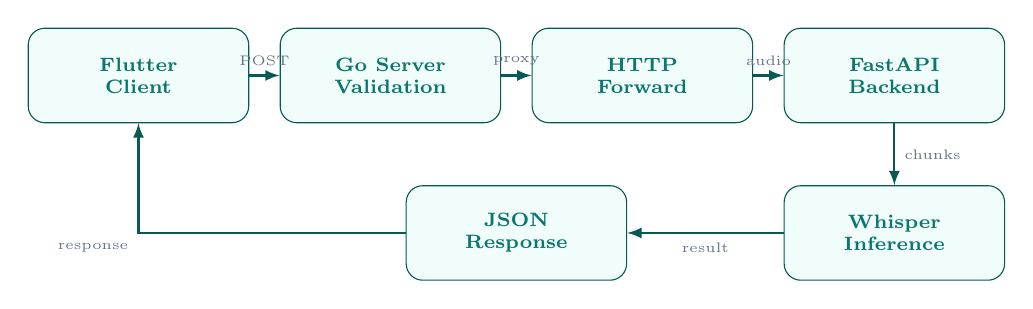
\begin{tikzpicture}[
  flownode/.style={
    draw=teal!60!black, rounded corners=6pt, minimum width=2.8cm,
    minimum height=1.2cm, fill=tealbg, font=\scriptsize\bfseries,
    text=teal!80!black, align=center
  },
  arrow/.style={-latex, thick, teal!60!black},
  label/.style={font=\tiny, color=slategray}
]

\node[flownode] (s1) at (0, 0) {Flutter\\Client};
\node[flownode] (s2) at (3.2, 0) {Go Server\\Validation};
\node[flownode] (s3) at (6.4, 0) {HTTP\\Forward};
\node[flownode] (s4) at (9.6, 0) {FastAPI\\Backend};
\node[flownode] (s5) at (9.6, -2) {Whisper\\Inference};
\node[flownode] (s6) at (4.8, -2) {JSON\\Response};

\draw[arrow] (s1) -- node[label, above] {POST} (s2);
\draw[arrow] (s2) -- node[label, above] {proxy} (s3);
\draw[arrow] (s3) -- node[label, above] {audio} (s4);
\draw[arrow] (s4) -- node[label, right] {chunks} (s5);
\draw[arrow] (s5) -- node[label, below] {result} (s6);
\draw[arrow] (s6) -| node[label, below left] {response} (s1);

\end{tikzpicture}
\caption{Request lifecycle flow diagram}
\label{fig:request_lifecycle}
\end{figure}

% ═══════════════════════════════════════════════════════════════════════════════
% CHAPTER 12: FAILURE HANDLING
% ═══════════════════════════════════════════════════════════════════════════════
\chapter{Failure Handling}

\section{Error Propagation Model}

The Tahkik server implements a layered error handling strategy where failures at each stage are caught, wrapped with contextual information, and propagated as structured JSON responses to the client.

\begin{table}[H]
  \centering
  \caption{Failure scenarios and server responses}
  \label{tab:failure_scenarios}
  \renewcommand{\arraystretch}{1.3}
  \begin{tabular}{lcp{6.5cm}}
    \toprule
    \textbf{Failure Scenario} & \textbf{HTTP Code} & \textbf{Behaviour} \\
    \midrule
    Invalid HTTP method & 405 & Go server rejects immediately \\
    Missing audio field & 400 & Go server returns ``missing 'audio' field'' \\
    Unsupported format & 400 & Go server returns ``unsupported audio format'' \\
    Multipart parse failure & 400 & Go server returns parse error details \\
    Inference server unreachable & 500 & Go HTTP client returns connection error \\
    Inference timeout (5\,min) & 500 & Go HTTP client returns timeout error \\
    Model inference exception & 500 & Python returns error JSON; Go forwards it \\
    \bottomrule
  \end{tabular}
\end{table}

\section{Inference Backend Unavailability}

When the inference backend is unreachable (e.g., HF Space is sleeping, network failure, or the local Python server is not running), the Go server's HTTP client returns a connection error. This is caught in the \texttt{RunInference} function and returned to the client as:

\begin{warnbox}[title=Backend Unavailable Response]
\begin{verbatim}
{
  "status": "error",
  "message": "inference request: dial tcp: connect: connection refused"
}
\end{verbatim}
\end{warnbox}

\section{Timeout Handling}

The Go inference client enforces a 5-minute timeout (\texttt{http.Client\{Timeout: 5 * time.Minute\}}). If the inference backend does not respond within this window --- for example, due to an exceptionally long audio file or a cold-start delay on the HF Space --- the client aborts the request and returns a timeout error to the caller.

\section{WebSocket Failure Recovery}

The WebSocket streaming endpoint implements additional resilience mechanisms:

\begin{emeraldbox}[title=WebSocket Resilience]
\begin{itemize}
  \item \textbf{Task cancellation}: On client disconnect, all pending background inference tasks are explicitly cancelled via \texttt{task.cancel()}, preventing orphaned coroutines from holding the inference lock.
  \item \textbf{Generation counter}: Each session reset increments a generation counter. Background tasks compare their generation to the current value before writing results, ensuring stale outputs are silently discarded.
  \item \textbf{Graceful close}: The \texttt{finally} block guarantees cleanup of all pending tasks and socket closure, regardless of how the connection terminates.
  \item \textbf{Exception isolation}: Individual inference errors within partial transcription tasks are caught and logged without terminating the WebSocket connection, allowing the session to continue.
\end{itemize}
\end{emeraldbox}

% ═══════════════════════════════════════════════════════════════════════════════
% CHAPTER 13: LOGGING AND MONITORING
% ═══════════════════════════════════════════════════════════════════════════════
\chapter{Logging and Monitoring}

\section{Current Logging Implementation}

Both server components produce structured log output to standard output, enabling integration with container log aggregation systems.

\begin{table}[H]
  \centering
  \caption{Logging behaviour by component}
  \label{tab:logging}
  \renewcommand{\arraystretch}{1.3}
  \begin{tabular}{llp{7cm}}
    \toprule
    \textbf{Component} & \textbf{Mechanism} & \textbf{Information Logged} \\
    \midrule
    Go server & \texttt{log.Printf} & Startup (port, backend URL), request errors, server-level failures \\
    Python (local) & \texttt{print()} with \texttt{[inference]} prefix & Model loading stages, device selection, readiness signal, request errors \\
    FastAPI (HF Space) & \texttt{print()} with \texttt{[inference]} / \texttt{[ws]} prefix & Model loading, WebSocket connect/disconnect, partial transcription progress, session resets, errors with full tracebacks \\
    \bottomrule
  \end{tabular}
\end{table}

\section{Log Output Examples}

\begin{lstlisting}[caption={Typical Go server startup log}]
inference backend: https://benhadjermed-tahkik-inference.hf.space
Tahkik server listening on :8080
\end{lstlisting}

\begin{lstlisting}[caption={Typical Python inference server log}]
[inference] importing libraries...
[inference] using device: cpu
[inference] downloading/loading processor (openai/whisper-base)...
[inference] processor ready
[inference] loading faster-whisper model...
[inference] model ready
[ws] client connected
[ws] partial: <transcription text>...
[ws] stop received, buffer size: 320000 bytes
[ws] client disconnected
[ws] connection closed
\end{lstlisting}

\section{Proposed Monitoring Enhancements}

\begin{goldbox}[title=Recommended Monitoring Stack]
\begin{itemize}
  \item \textbf{Prometheus metrics}: Expose \texttt{/metrics} endpoint on the Go server with counters for total requests, error rates, and histograms for request latency and audio file sizes.
  \item \textbf{Grafana dashboards}: Visualise inference latency distributions, request throughput, error rate trends, and WebSocket connection counts in real-time.
  \item \textbf{Structured logging}: Migrate from plain-text \texttt{print()} statements to JSON-structured logs (e.g., via Python's \texttt{structlog} or Go's \texttt{slog}), enabling efficient parsing and filtering in log aggregation platforms.
  \item \textbf{Health check monitoring}: Implement periodic external health probes against \texttt{/health} to detect and alert on inference backend unavailability.
  \item \textbf{Request tracing}: Introduce correlation IDs (e.g., UUID per request) propagated from the Go server to the Python backend, enabling end-to-end request tracing across both services.
\end{itemize}
\end{goldbox}

% ═══════════════════════════════════════════════════════════════════════════════
% CONCLUSION
% ═══════════════════════════════════════════════════════════════════════════════
\chapter{Conclusion}

\section{Summary}
This report documented the complete server-side infrastructure of the Tahkik project, covering the Go API gateway, Python inference backends (local and production), WebSocket streaming protocol, HF Space deployment, and API contracts. The proxy architecture ensures clean separation of concerns between client-facing and ML-facing components.

\section{Key Features}
\begin{emeraldbox}[title=System Capabilities]
\begin{itemize}
  \item Dual-mode inference: local PyTorch server for development, faster-whisper CTranslate2 INT8 for production
  \item Real-time WebSocket streaming with sliding-window partial transcription
  \item Hallucination filtering for Arabic Whisper outputs
  \item Docker-based deployment to Hugging Face Spaces with zero infrastructure management
  \item Automatic CTranslate2 model conversion with INT8 quantization
  \item 50\,MB audio upload support with multi-format compatibility
\end{itemize}
\end{emeraldbox}

\section{Future Enhancements}
\begin{goldbox}[title=Planned Extensions]
\begin{itemize}
  \item \textbf{GPU Acceleration}: Deploy with T4/A100 GPU for sub-second inference latency
  \item \textbf{Batch Processing}: Support concurrent audio evaluations with request queuing
  \item \textbf{Model Versioning}: Hot-swap model checkpoints without server restart
  \item \textbf{Caching}: Cache frequently recited ayah transcriptions for instant responses
  \item \textbf{Monitoring}: Add Prometheus metrics for inference latency and error rates
\end{itemize}
\end{goldbox}

\begin{emeraldbox}[title=Closing Statement]
\begin{center}
\large\itshape
``The best architecture is one that makes the complex simple.''\\[6pt]
\normalsize\normalfont\color{slategray} --- Software Engineering Principle
\end{center}
\vspace{6pt}
\normalsize
The Tahkik server infrastructure demonstrates that a well-designed proxy architecture can effectively bridge mobile applications with state-of-the-art machine learning models while maintaining simplicity, reliability, and ease of deployment.
\end{emeraldbox}

% ═══════════════════════════════════════════════════════════════════════════════
% REFERENCES
% ═══════════════════════════════════════════════════════════════════════════════
\chapter*{References}
\addcontentsline{toc}{chapter}{References}

\begin{enumerate}[label={[\arabic*]}]
  \item A. Radford et al., ``Robust Speech Recognition via Large-Scale Weak Supervision,'' \textit{arXiv preprint arXiv:2212.04356}, 2022.
  \item Hugging Face, ``Transformers: State-of-the-art Machine Learning for PyTorch, TensorFlow, and JAX,'' \url{https://github.com/huggingface/transformers}.
  \item SYSTRAN, ``faster-whisper: Faster Whisper transcription with CTranslate2,'' \url{https://github.com/SYSTRAN/faster-whisper}.
  \item The Go Programming Language, \url{https://golang.org}.
  \item FastAPI Framework, \url{https://fastapi.tiangolo.com}.
  \item Hugging Face Spaces Documentation, \url{https://huggingface.co/docs/hub/spaces}.
  \item CTranslate2, ``Fast inference engine for Transformer models,'' \url{https://github.com/OpenNMT/CTranslate2}.
\end{enumerate}


\end{document}
